\chapter{Psalm 34}

\begin{figure}
  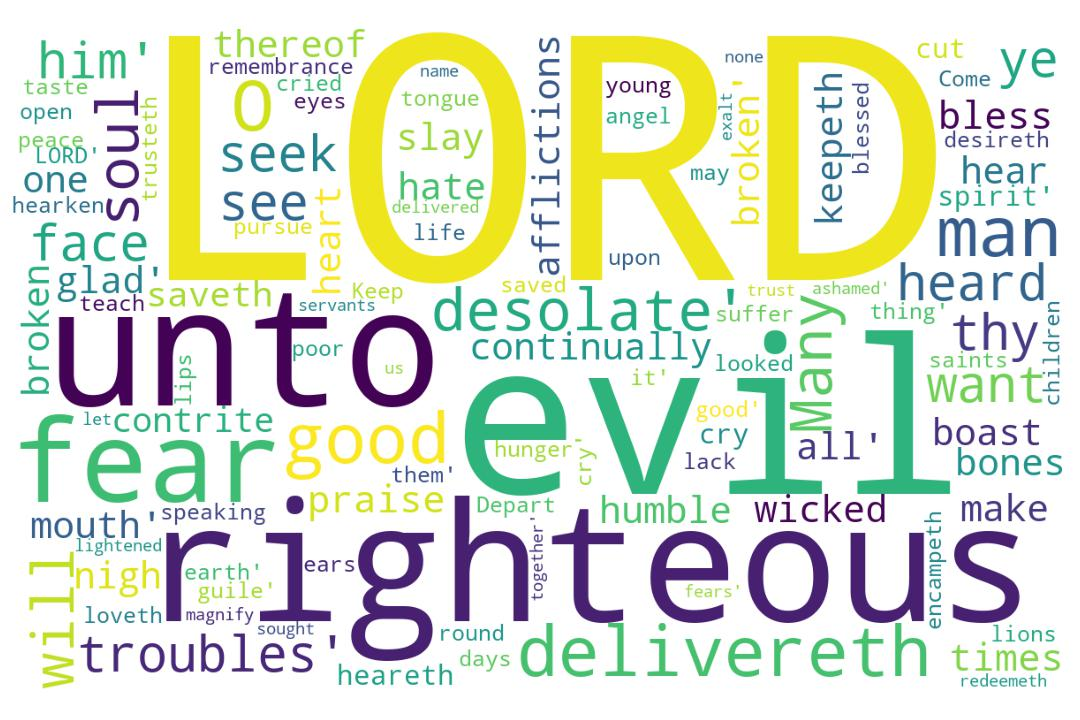
\includegraphics[width=\linewidth]{19OT-Psalms/Psalm34-WordCloud.jpg}
  \caption{Psalm 34 Word Cloud}
  \label{fig:Psalm 34 word Cloud}
\end{figure}


\marginpar{\scriptsize \centering \fcolorbox{bone}{lime}{\textbf{A FAITH WORTH HAVING}}\\ (Psalm 34:1--22) 
\begin{compactenum}[I.][8]
    \item In One I can \textbf{Continually Praise} the Lord \index[scripture]{Psalms!Psa 034:01}(Psa 34:1)
    \item In One that is \textbf{Constantly Present} \index[scripture]{Psalms!Psa 034:01}(Psa 34:1)
    \item In One who \textbf{Considers my Pleas} \index[scripture]{Psalms!Psa 034:06}(Psa 34:6)
    \item In one who is \textbf{Certifiably Proven} \index[scripture]{Psalms!Psa 034:08}(Psa 34:8)
    \item In whom I Get \textbf{Unceasing Provision} \index[scripture]{Psalms!Psa 034:09}(Psa 34:9)
    \item In whom who Provides \textbf{Comforting Proximity} \index[scripture]{Psalms!Psa 034:18}(Psa 34:18)
\end{compactenum} }

\marginpar{\scriptsize \centering \fcolorbox{bone}{yellow}{\textbf{IMPERATIVES FOR THE BELIEVER}}\\ (Psalm 34:1--22) 
\begin{compactenum}[I.][8]
    \item \textbf{Bless} the Lord \index[scripture]{Psalms!Psa 034:01}(Psa 34:1)
    \item \textbf{Praise} the Lord \index[scripture]{Psalms!Psa 034:01}(Psa 34:1)
    \item \textbf{Boast} of the Lord \index[scripture]{Psalms!Psa 034:02}(Psa 34:2)
    \item \textbf{Magnify} the Lord \index[scripture]{Psalms!Psa 034:03}(Psa 34:3)
    \item \textbf{Exalt} the Lord \index[scripture]{Psalms!Psa 034:03}(Psa 34:3)
    \item \textbf{Seek} the Lord \index[scripture]{Psalms!Psa 034:04}(Psa 34:4)
    \item \textbf{Taste} the Lord \index[scripture]{Psalms!Psa 034:08}(Psa 34:8)
    \item \textbf{Trust} in the Lord \index[scripture]{Psalms!Psa 034:08}(Psa 34:8)
\end{compactenum}}

\marginpar{\scriptsize \centering \fcolorbox{bone}{black}{\textbf{\textcolor[cmyk]{0,0,0,0}{AN INVOLVED GOD}}}\\ (Psalm 34) 
\begin{compactenum}[I.][8]
    \item He \textbf{Enlightens} his People \index[scripture]{Psalms!Psa 034:05} (Psa 34:5)
    \item He \textbf{Lingers} Nearby \index[scripture]{Psalms!Psa 034:07}\index[scripture]{Psalms!Psa 034:18} (Psa 34:7, 18)
    \item He is \textbf{Longing} to Bless \index[scripture]{Psalms!Psa 034:10}(Psa 34:10)
    \item He is \textbf{Looking} at the Saints \index[scripture]{Psalms!Psa 034:15}(Psa 34:15)
    \item He is \textbf{Listening} for their Prayers \index[scripture]{Psalms!Psa 034:15}(Psa 34:15)
    \item He is \textbf{Looming} against Evil\index[scripture]{Psalms!Psa 034:16}(Psa 34:16)
\end{compactenum} }

\footnote{\textcolor[cmyk]{0.99998,1,0,0}{\hyperlink{TOC}{Return to end of Table of Contents.}}}\footnote{\href{https://www.audioverse.org/english/audiobibles/books/ENGKJV/O/Ps/1}{\textcolor[cmyk]{0.99998,1,0,0}{Psalms Audio}}}\textcolor[cmyk]{0.99998,1,0,0}{\emph{A Psalm} of David, when he changed his behaviour before Abimelech; who drove him away, and he departed.}\footnote{\textbf{1 Samuel 21:10} - And David arose, and fled that day for fear of Saul, and went to Achish the king of Gath.}\\
\\
\textcolor[cmyk]{0.99998,1,0,0}{I will bless the LORD \fcolorbox{bone}{lime}{at all times}: his praise \emph{shall} \fcolorbox{bone}{lime}{continually} \emph{be} in my mouth.}
[2] \textcolor[cmyk]{0.99998,1,0,0}{My soul shall make her boast in the LORD: the humble shall hear \emph{thereof}, and be glad.}
[3] \textcolor[cmyk]{0.99998,1,0,0}{O magnify the LORD with me, and let us exalt his name together.}
[4] \textcolor[cmyk]{0.99998,1,0,0}{I sought the LORD, and he heard me, and delivered me from all my fears.}
[5] \textcolor[cmyk]{0.99998,1,0,0}{They looked unto him, and were lightened: and their faces were not ashamed.}
[6] \textcolor[cmyk]{0.99998,1,0,0}{This poor man cried, and \fcolorbox{bone}{lime}{the LORD heard} \emph{him}, and saved him out of all his troubles.}
[7] \textcolor[cmyk]{0.99998,1,0,0}{The angel of the LORD encampeth round about them that fear him, and delivereth them.}
[8] \textcolor[cmyk]{0.99998,1,0,0}{O \fcolorbox{bone}{lime}{taste and see} that the LORD \emph{is} good: blessed \emph{is} the man \emph{that} trusteth in him.}
[9] \textcolor[cmyk]{0.99998,1,0,0}{O fear the LORD, ye his saints: for \emph{there} \emph{is} \fcolorbox{bone}{lime}{no want} to them that fear him.}
[10] \textcolor[cmyk]{0.99998,1,0,0}{The young lions do lack, and suffer hunger: but they that seek the LORD shall not want any good \emph{thing}.}
[11] \textcolor[cmyk]{0.99998,1,0,0}{Come, ye children, hearken unto me: I will teach you the fear of the LORD.}
[12] \textcolor[cmyk]{0.99998,1,0,0}{What man \emph{is} \emph{he} \emph{that} desireth life, \emph{and} loveth \emph{many} days, that he may see good?}
[13] \textcolor[cmyk]{0.99998,1,0,0}{Keep thy tongue from evil, and thy lips from speaking guile.}
[14] \textcolor[cmyk]{0.99998,1,0,0}{Depart from evil, and do good; seek peace, and pursue it.}
[15] \textcolor[cmyk]{0.99998,1,0,0}{The eyes of the LORD \emph{are} upon the righteous, and his ears \emph{are} {open} unto their cry.}
[16] \textcolor[cmyk]{0.99998,1,0,0}{The face of the LORD \emph{is} against them that do evil, to cut off the remembrance of them from the earth.}
[17] \textcolor[cmyk]{0.99998,1,0,0}{\emph{The} \emph{righteous} cry, and the LORD heareth, and delivereth them out of all their troubles.}
[18] \textcolor[cmyk]{0.99998,1,0,0}{The LORD \emph{is} \fcolorbox{bone}{lime}{nigh unto them} that are of a broken heart; and saveth such as be of a contrite spirit.}
[19] \textcolor[cmyk]{0.99998,1,0,0}{Many \emph{are} the afflictions of the righteous: but the LORD delivereth him out of them all.}
[20] \textcolor[cmyk]{0.99998,1,0,0}{He keepeth all his bones: not one of them is broken.}
[21] \textcolor[cmyk]{0.99998,1,0,0}{Evil shall slay the wicked: and they that hate the righteous shall be desolate.}
[22] \textcolor[cmyk]{0.99998,1,0,0}{The LORD redeemeth the soul of his servants: and none of them that trust in him shall be desolate.}